\documentclass[10pt,a4paper]{article}

\usepackage[utf8]{inputenc}
\usepackage[T1]{fontenc}
\usepackage{amsmath,amssymb,amsfonts}
\usepackage{graphicx}
\usepackage{hyperref}
\usepackage{algorithm}
\usepackage{algpseudocode}
\usepackage{geometry}
\usepackage{cite}

% Page layout
\geometry{margin=1.5cm}

% Title page
\title{\Large\textbf{PixelBytes: Catching Unified Embedding for Multimodal Generation}}
\author{\large Fabien Furfaro}
\date{\large 2024}

\begin{document}

\maketitle


\begin{abstract}
This report introduces PixelBytes Embedding, a novel approach for unified multimodal representation learning. Our method captures diverse inputs in a single, cohesive representation, enabling emergent properties for multimodal sequence generation, particularly for text and pixelated images. Inspired by state-of-the-art sequence models such as Image Transformers, PixelCNN, and Mamba-Bytes, PixelBytes aims to address the challenges of integrating different data types. We explore various model architectures, including Recurrent Neural Networks (RNNs), State Space Models (SSMs), and Attention-based models, focusing on bidirectional processing and our innovative PxBy embedding technique. Our experiments, conducted on a specialized PixelBytes Pokémon dataset, demonstrate that bidirectional sequence models with PxBy embedding and convolutional layers can generate coherent multimodal sequences. This work contributes to the advancement of integrated AI models capable of understanding and generating multimodal data in a unified manner. Code is available at \url{https://github.com/fabienfrfr}.
\end{abstract}

\let\thefootnote\relax\footnotetext{$^{*}$ Corresponding author: Fabien Furfaro (\url{fabien.furfaro@gmail.com}).}


\begin{figure}[h]
\centering
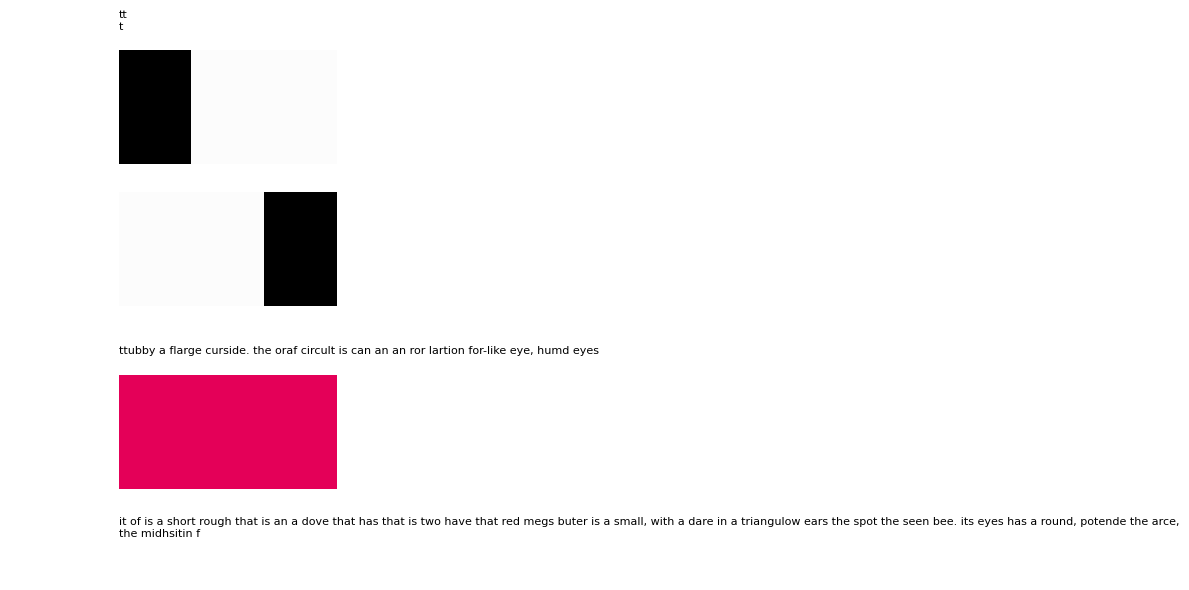
\includegraphics[width=0.8\linewidth]{example_generation.png}
\caption{Example of a PixelBytes-generated Pokémon and its description. Left: Generated pixelated image. Right: Corresponding text description. The red box indicates the model's attention window for both pixels and words. Note that the model currently exhibits some inaccuracies in image generation and occasionally invents words, highlighting areas for future improvement.}
\label{fig:example_generation}
\end{figure}

\section{Introduction}

Recent advancements in artificial intelligence have led to increasingly generalist models, not by combining multiple specialized components, but by giving simple tasks to models where emergent properties—complex behaviors that arise from simpler underlying rules—appear. This is the case with generative language models like GPT \cite{brown2020language}. However, these models are limited by their focus on language alone, failing to capture the full complexity of multimodal understanding \cite{alayrac2023language}. To address this limitation, researchers have explored combining LLMs with other modalities \cite{radford2021learning, ramesh2022hierarchical}. But this brings us back to the initial problem, as it often results in specialized model combinations without allowing for new emergent properties. We propose "PixelBytes Embedding", a novel approach enabling unified training across modalities by capturing diverse inputs in a single, cohesive representation.

Multimodal sequence generation, which involves the creation of coherent outputs combining various data types such as text, images, and numerical sequences, presents a significant challenge in artificial intelligence \cite{baltrusaitis2019multimodal}. While models like GPT have excelled in text generation \cite{brown2020language}, there's a growing need for unified approaches that can seamlessly handle varied data types. Building upon these findings, PixelBytes aims to address the challenge of unified text and image generation by proposing a model capable of producing mixed sequences of text and images in a coherent and unified manner. We draw inspiration from state-of-the-art sequence models, including Image Transformers \cite{parmar2018image}, PixelCNN \cite{oord2016conditional}, and recent developments in bytes generation by mamba architectures \cite{wang2024mamba}.

Our research explores various architectures including Recurrent Neural Networks (RNNs), State Space Models (SSMs), and Attention-based models, focusing on the effectiveness of bidirectional processing \cite{gu2023visual, gu2023bidirectional}, novel embedding techniques (particularly PxBy embedding, which unifies pixel and byte-level representations), the impact of convolutional layers, effects of model depth, input dimensionality, and size. Our experiments reveal that bidirectional sequence models with PxBy embedding and convolutional layers demonstrate good performance in generating coherent sequences.

Our results show that it is possible to train sequence models with unified embeddings for both text and pixel completion. This paper presents our methodology to construct unified sequence data from text and image, experimental results, and analysis, contributing to the development of our sequence generation embedding models. The proposed PixelBytes Embedding approach has the potential to significantly advance the field of multimodal AI, enabling more integrated and versatile models capable of understanding and generating diverse types of data. This could lead to improvements in areas such as visual question answering, image captioning, and multimodal content generation for virtual and augmented reality applications.

\section{Model Architecture}

\subsection{Overview}
The PixelBytes architecture is designed to seamlessly integrate multimodal data for unified sequence generation. At its core, the model incorporates two key innovative components: a specialized tokenizer sequence constructor and a unified multimodal embedding technique called PxByEmbed. The tokenizer sequence constructor is engineered to process both pixelated images and text at a byte level, enabling a consistent representation across modalities. This is complemented by PxByEmbed, our novel embedding approach that creates a unified representation for both pixel and byte data in a single, coherent space. This architecture draws inspiration from recent advancements in multimodal learning \cite{baltrusaitis2019multimodal} and efficient sequence modeling \cite{vaswani2017attention}, allowing PixelBytes to capture intrinsic relationships between visual and textual information effectively.

\subsection{Dataset Construction}

Image captioning datasets, while combining visual and textual modalities, prove unsuitable for joint text and image generation due to limited text content and difficulties in interpreting pixelated versions of high-resolution images. To address these limitations, we developed a specialized Pokémon dataset, offering advantages such as a long-standing franchise history, pixelated designs, rich descriptive text, and over 1000 unique Pokémon. This aligns with trends in creating specialized datasets for multimodal learning \cite{lin2014microsoft}. 

We constructed our dataset by web scraping Pokémon miniatures and descriptions from Pokepedia using Beautiful Soup \cite{richardson2007beautiful}, maintaining a 2/3 text to 1/3 image ratio. For image quantization, we employed a 55-color palette inspired by the NES, creating tokens representing different color combinations. This approach translates visual information into a format suitable for sequence modeling, similar to recent work in discrete representation learning for images \cite{van2017neural}. The quantization and pixelization process used OpenCV and scikit-image \cite{bradski2000opencv, vanderwalt2014scikit}. To ensure balanced representation, we adjusted the number of image and text tokens to 113 characters for each modality, allowing the model to learn equally from both visual and textual information. The final dataset, balancing text and pixelated images, is available on the Hugging Face Datasets Hub for reproducibility at \url{https://huggingface.co/datasets/ffurfaro/PixelBytes-Pokemon}.

\section{Multimodal Embedding Algorithm}

\subsection{PxByEmbed: Multimodal Embedding Algorithm}

At the core of our approach is the PxByEmbed algorithm, which represents mixed sequences of text and pixelated images in a unified manner. This algorithm builds upon existing embedding techniques by incorporating spatial adaptivity, allowing for representation of both textual and visual information. PxByEmbed is designed to address the specific needs of pixel-level image representation and byte-level text encoding. The algorithm uses a learned embedding matrix to map each token (text or image) to a vector space, while maintaining spatial relationships for image tokens. This approach allows our model to handle both modalities within a single framework.

\begin{algorithm}[h]
\caption{PxByEmbed: Multimodal Embedding Algorithm (k=3)
\newline
\textbf{Input:} $V$: vocabulary size, $D$: embedding dimension
\newline
\textbf{Output:} Embedded representation $\mathbf{E} \in \mathbb{R}^{B \times L \times D}$
\newline
\textbf{Note:} $\mathbf{X}_{emb} \in \mathbb{R}^{B \cdot L \times E_{int} \times k \times k}$, 
$\mathbf{X}_{flat} \in \mathbb{R}^{B \cdot L \times E_{int}k^2}$, 
$\mathbf{X}_{proj} \in \mathbb{R}^{B \cdot L \times D}$
}
\begin{algorithmic}[0]
\State \textbf{Initialize:}
\State $k \gets 3$
\State $E_{int} \gets \max(9, \lfloor D / k^2 \rfloor)$
\State $\mathbf{\alpha} \in \mathbb{R}^{1 \times 1 \times k \times k}$ 
\State $\mathbf{W}_{emb} \in \mathbb{R}^{V \times E_{int}}$ 
\State $\mathbf{W}_{proj} \in \mathbb{R}^{E_{int}k^2 \times D}$ 
\State $\mathbf{W}_{patch} \in \mathbb{R}^{E_{int} \times E_{int} \times k \times k}$ 

\Function{PxByEmbed}{$\mathbf{X} \in \mathbb{Z}^{B \times L \times k \times k}$}
    \State $\mathbf{X}_{emb} \gets \text{Permute}(\text{Embed}(\mathbf{X}, \mathbf{W}_{emb}), [0, 3, 1, 2])$ 
    
    \State $\mathbf{X}_{patch} \gets \text{Conv2D}(\mathbf{X}_{emb}, \mathbf{W}_{patch}, \text{padding}=1)$
    \State $\mathbf{X}_{combined} \gets \sigma(\mathbf{\alpha}) \odot \mathbf{X}_{emb} + (1 - \sigma(\mathbf{\alpha})) \odot \mathbf{X}_{patch}$
    
    \State $\mathbf{X}_{flat} \gets \text{Flatten}(\mathbf{X}_{combined})$ 
    \State $\mathbf{X}_{proj} \gets \mathbf{X}_{flat}\mathbf{W}_{proj}$ 
    \State $\mathbf{E} \gets \text{LayerNorm}(\mathbf{X}_{proj})$
    \State $\mathbf{E} \gets \text{Reshape}(\mathbf{E}, [B, L, D])$
    \State \Return $\mathbf{E}$
\EndFunction
\end{algorithmic}
\end{algorithm}

\subsection{Managing Transitions}

PixelBytes uses a method to handle transitions between text and image tokens during sequence generation. This approach is used in both dataset construction and sequence generation (Figure \ref{fig:example_generation}).

For dataset construction, we use a 2D input sequence method with a 3x3 context window around each token. We use special tokens to mark transitions between text and images, and add padding to keep context sizes consistent. For text, only previous tokens are included in the context windows. The \texttt{input\_seq\_construct} function implements this process.

During sequence generation, the \texttt{\_process\_token} function manages transitions. It handles text tokens (bytes) and image tokens (tuples) differently, and takes care of special characters like newlines and tabs. A \texttt{sequence\_clock} keeps track of the generation progress. Each new token's context is represented in a 3x3 matrix, which helps maintain coherence when switching between text and images.

\section{Training and Evaluation}

\subsection{Model Architectures}
We evaluated three compact model architectures, each with fewer than 100,000 parameters: a Recurrent Neural Network (RNN) using bidirectional Long Short-Term Memory (LSTM) units \cite{hochreiter1997long}, a Transformer \cite{vaswani2017attention}, and Mamba, based on the State Space Model (SSM) \cite{gu2022efficiently}. These models were adapted to process our dataset of pixel data and bytecode sequences. Training was conducted on Kaggle using dual T4 GPUs, with a batch size of 32, sequence length of 256, stride size of 32, and learning rate of 0.001. We trained for 200 epochs, evaluating performance every 5 epochs. The resulting models are available at \url{https://huggingface.co/ffurfaro/PixelBytes-Pokemon}. Additionally, we developed a more specialized model for generation tasks, which is not presented in this paper.

\begin{figure}[htbp]
\centering
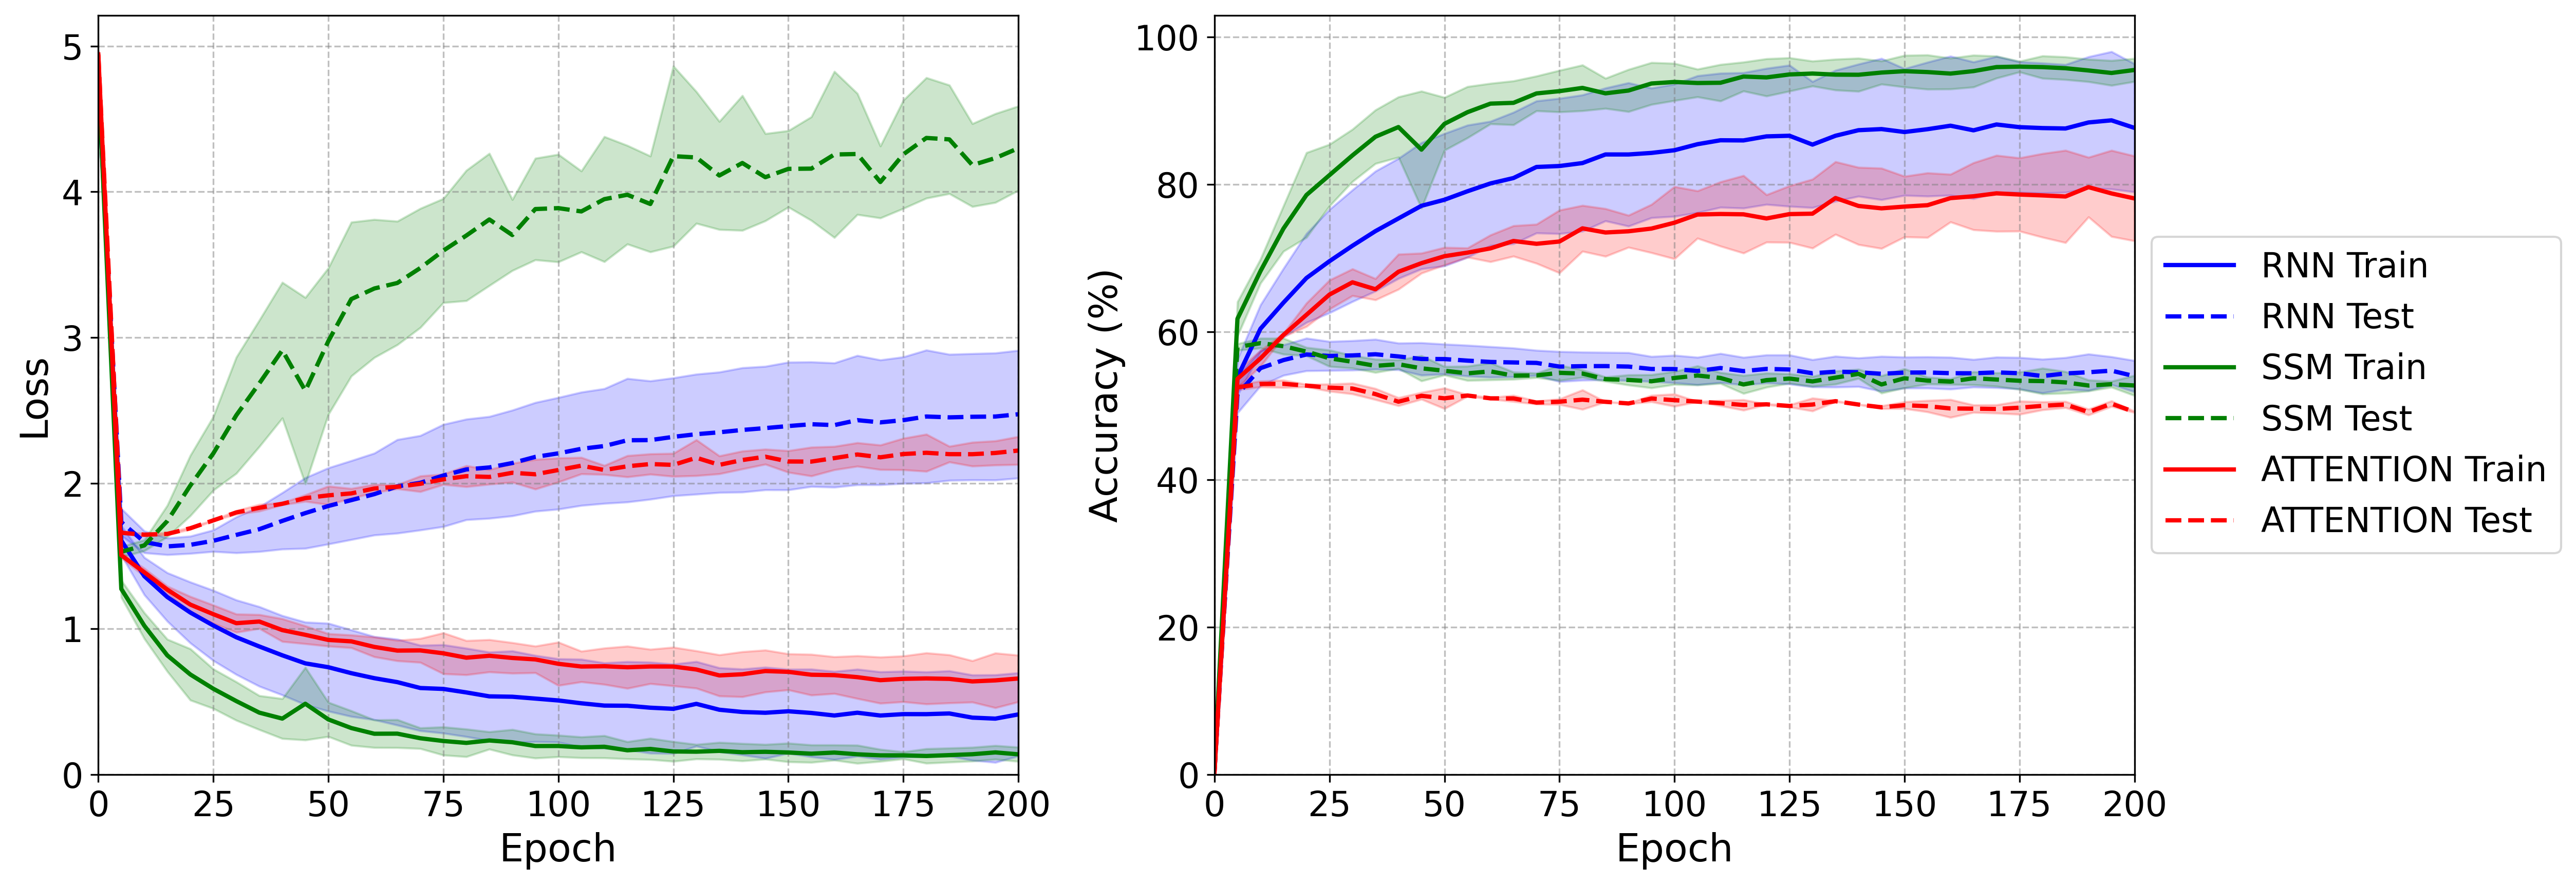
\includegraphics[width=\textwidth]{training_results.png}
\caption{Training and validation metrics (Loss, Accuracy) for RNN, Transformer, and SSM models over 200 epochs.}
\label{fig:training_results}
\end{figure}

Figure \ref{fig:training_results} shows the training and validation metrics for our three model types over 200 epochs. The State Space Models (SSM) achieved the best scores for loss and accuracy. However, the widening gap between their training and validation curves suggests they may be overfitting, meaning they learned the training data well but struggled to generalize to new examples.

In contrast, the LSTMs (referred to as RNNs in our analysis) demonstrated more balanced performance. The closer alignment of their training and validation curves indicates they may generalize better to unseen data. The Transformer model had the lowest performance among the three. This could be due to the absence of positional encoding trick, which is important for Transformers in sequence tasks.

Overall, these results highlight the strengths and weaknesses of each model type. While SSMs showed strong training performance, their tendency to overfit suggests that additional regularization techniques might be needed. The stable performance of RNNs indicates their suitability for our task, as they balance well between fitting the training data and generalizing to new data. The Transformer's performance suggests it may require further adjustments to improve its effectiveness for this task.

\subsection{Generation Evaluation Metrics}

We tested different model types including State Space Models (SSM), Attention models (Att), and Recurrent Neural Networks (RNN) for generating 16 consecutive sequences. We used three metrics to evaluate their performance: Hamming Distance, Cosine Similarity, and BLEU Score \cite{sutskever2014sequence, hamming1950error, papineni2002bleu}.

\begin{table}[h]
\centering
\small
\begin{tabular}{cccccccccc}
\hline
Type & Dir. & Emb. & Conv. & In Emb & Hidden State & Depth & Hamming & Cosine & BLEU \\
\hline
SSM & Bi & PxBy & Y & 81 & 64 & 1 & 0.170 $\pm$ 0.086 & 0.883 $\pm$ 0.105 & 0.753 $\pm$ 0.115 \\
SSM & Bi & PxBy & Y & 81 & 64 & 2 & 0.158 $\pm$ 0.074 & 0.896 $\pm$ 0.095 & 0.771 $\pm$ 0.097 \\
SSM & Uni & PxBy & Y & 81 & 64 & 2 & 0.166 $\pm$ 0.081 & 0.886 $\pm$ 0.102 & 0.760 $\pm$ 0.106 \\
Att & - & PxBy & Y & 81 & 64 & 1 & 0.157 $\pm$ 0.064 & 0.887 $\pm$ 0.103 & 0.765 $\pm$ 0.088 \\
Att & - & PxBy & Y & 81 & 64 & 2 & 0.159 $\pm$ 0.066 & 0.887 $\pm$ 0.103 & 0.760 $\pm$ 0.092 \\
RNN & Bi & Center & N & 81 & 64 & 2 & 0.185 $\pm$ 0.074 & 0.888 $\pm$ 0.083 & 0.750 $\pm$ 0.093 \\
RNN & Bi & PxBy & Y & 81 & 64 & 2 & 0.153 $\pm$ 0.061 & 0.902 $\pm$ 0.090 & 0.777 $\pm$ 0.083 \\
RNN & Bi & PxBy & Y & 162 & 64 & 2 & 0.152 $\pm$ 0.062 & 0.905 $\pm$ 0.089 & 0.778 $\pm$ 0.084 \\
RNN & Bi & PxBy & Y & 36 & 64 & 2 & 0.152 $\pm$ 0.061 & 0.904 $\pm$ 0.090 & 0.778 $\pm$ 0.083 \\
RNN & Bi & PxBy & Y & 81 & 128 & 2 & 0.153 $\pm$ 0.063 & 0.903 $\pm$ 0.091 & 0.776 $\pm$ 0.086 \\
RNN & Bi & PxBy & Y & 81 & 32 & 2 & \textbf{0.149} $\pm$ 0.062 & 0.899 $\pm$ 0.095 & \textbf{0.785} $\pm$ 0.082 \\
RNN & Bi & PxBy & Y & 81 & 64 & 1 & 0.149 $\pm$ 0.062 & 0.897 $\pm$ 0.096 & 0.780 $\pm$ 0.085 \\
RNN & Bi & PxBy & Y & 81 & 64 & 3 & 0.153 $\pm$ 0.063 & \textbf{0.906} $\pm$ 0.087 & 0.776 $\pm$ 0.086 \\
RNN & Bi & PxBy & N & 81 & 64 & 2 & 0.151 $\pm$ 0.062 & 0.903 $\pm$ 0.090 & 0.779 $\pm$ 0.084 \\
RNN & Uni & PxBy & Y & 81 & 64 & 2 & 0.153 $\pm$ 0.064 & 0.904 $\pm$ 0.088 & 0.777 $\pm$ 0.087 \\
\hline
\end{tabular}
\caption{Comparison of model characteristics and performance (mean $\pm$ std)}
\label{tab:model_comparison}
\end{table}

The results show that RNN models with PxBy embedding generally perform better than other types. The best Hamming distance (0.149 $\pm$ 0.062) and BLEU score (0.785 $\pm$ 0.082) come from the bidirectional PxBy RNN model with convolution, 81 embedding dimensions, and 32 hidden state dimensions. This suggests that a smaller hidden state in the RNN model can effectively capture sequence patterns.

The highest cosine similarity (0.906 $\pm$ 0.087) is from the 3-layer RNN model, indicating that more layers can improve sequence alignment. Adding convolution usually improves RNN model performance. Interestingly, changing the embedding dimension (36, 81, 162) in RNN models didn't affect performance much, suggesting these models can handle different embedding sizes well. The center embedding in RNNs didn't perform as well as PxBy embedding for this task.

\section{Results and Discussion}

Our experiments with various model architectures tested the effectiveness of unified text and image generation. We evaluated model performance using Hamming distance, cosine similarity, and BLEU score \cite{papineni2002bleu}. Bidirectional RNN models using PixelBytes (PxBy) embedding with convolutional layers generally performed better across our metrics. The PxBy embedding improved the mean BLEU score from 0.750 to 0.777 compared to a center-only approach, indicating its effectiveness in representing multimodal data. This finding aligns with recent work emphasizing the importance of effective multimodal embeddings in text-to-image generation tasks \cite{yan2024multimodal}.

Bidirectional models showed a slight advantage over unidirectional ones, with BLEU scores of 0.777 and 0.776 respectively. This suggests that bidirectionality may help capture sequential dependencies, consistent with other studies in sequence modeling \cite{schuster1997bidirectional}. Notably, varying state dimensions (32, 64, 128) had minimal impact on performance, with BLEU scores ranging from 0.775 to 0.784. While RNN models showed strong performance in our experiments, State Space Models (SSM) demonstrated rapid convergence during training, suggesting potential for future exploration in multimodal data processing. This is in line with recent advancements in SSM for sequence modeling tasks \cite{gu2022efficiently}.

\section{Conclusion and Future Work}

This study on PixelBytes highlights the potential for unified text-image generation, contributing to the growing field of multimodal AI \cite{baltrusaitis2019multimodal}. The performance of bidirectional RNN models with PxBy embedding underscores the importance of capturing both spatial and contextual information in multimodal data. Future work could focus on refining the PxByEmbed algorithm, testing on larger and more diverse datasets, exploring creative applications of multimodal generation, and further optimizing SSM and Attention models. These efforts aim to advance multimodal sequence modeling and generation techniques, addressing challenges identified in surveys of the field \cite{lin2014microsoft}.

\bibliographystyle{plain}
\bibliography{references}

\end{document}
